
\documentclass[a4paper,10pt]{article}

\usepackage{geometry}

\usepackage[utf8x]{inputenc}
\usepackage[bookmarks,colorlinks=false,pdfborder={0 0 0}]{hyperref}
\hypersetup{pdftitle={2. Praktikum: Technik und Technologie}}
\usepackage{url}
\usepackage[ngerman]{babel}
\usepackage{graphicx}
\usepackage{listings}

\parindent 0pt 
\parskip 10pt

\title{2. Praktikum: Technik und Technologie}
\author{Andreas Krohn \and Benjamin Vetter}

\begin{document}

\maketitle

\section{Kurzdokumentation}

Dem Quellcode liegt ein Ant Buildfile bei. 
Die Parameter \emph{Benutzername} und \emph{Port} sind über das Buildfile festgelegt.
Per \verb=ant run= wird die SIP Applikation kompiliert und gestartet.

Abbildung \ref{screenshot} zeigt einen Screenshot der gestarteten Anwendung. 

\begin{figure}[h]
	\begin{center}
		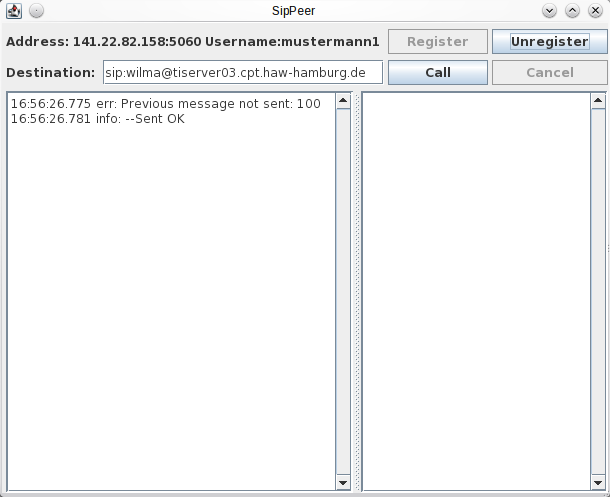
\includegraphics[width=0.75\textwidth]{screenshot_SipPeer.png}
	\end{center}

	\caption{Screenshot der Anwendung}

	\label{screenshot}
\end{figure}


Beim Start der SIP Applikation registriert diese sich beim SIP Proxy Server. Über die Buttons "`Unregister"' und "`Register"' kann diese Registrierung manuell zurückgezogen bzw. wieder gesetzt werden.

Die SIP Applikation kann sowohl UAC als auch UAS sein. 

Durch Betätigen des "`Call"'-Buttons wird eine Session zu dem im Textfeld angegebenen Teilnehmer aufgebaut. Damit übernimmt die Anwendung die UAC Rolle und setzt ein IGMP \verb=join= an die Gruppe \verb=239.238.237.17= ab. Eingehende Multicast Nachrichten werden in der Anwendung angezeigt. Der "`Cancel"'-Button beendet die Session und veranlasst das Verlassen der Multicast Gruppe.

Ruft ein anderer Teilnehmer die SIP Applikation an, übernimmt die Anwendung die UAS Rolle und beginnt kontinuierlich (1x pro Sekunde) Multicast Nachrichten zu senden bis die letzte Session beendet wird. Die Adressen der "`Anrufer"' werden für die Dauer der Session in der Anwendung angezeigt.


\section{Erklärung Ihrer Beobachtungen zur Multicast Paketverteilung}

\subsection{Wie erreichen die Multicast Daten Ihren Rechner auf der Ethernet Protokollebene?}

Hierzu werden die Multicast IP Host Group Adressen auf Ethernet Multicast Adressen gemappt,
indem die low-order 23 bit der IP-Adresse auf die low-order 23 bit der Ethernet Multicast Adressen gemappt werden (01-00-5E-00-00-00).
Da viele Ethernet-Netzwerkkarten bzgl. der konfigurierbaren Adressen, für die sie zuständig sein sollen, eingeschränkt sind, muss ggf. der Adress-Filter der Karte ausser Kraft gesetzt werden.
Hierdurch nimmt die Netzwerkkarte alle Pakete entgegen, auch wenn sie gar nicht für das Interface bestimmt sind (vgl. \url{http://tools.ietf.org/html/rfc1112} und Abbildung \ref{multicast_ethernet}).

\begin{figure}[h]
	\begin{center}
		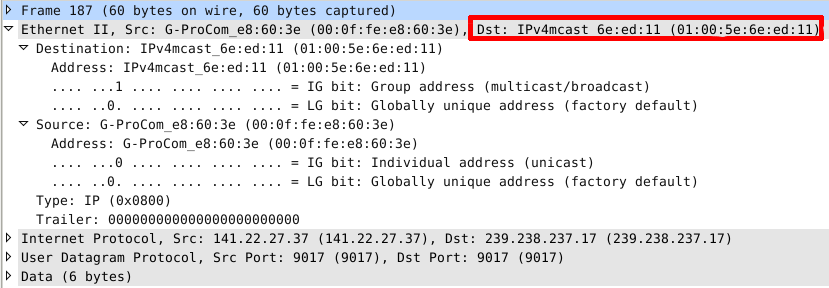
\includegraphics[width=1\textwidth]{multicast_ethernet.png}
	\end{center}

	\caption{Multicast im Ethernet}

	\label{multicast_ethernet}
\end{figure}

\subsection{Welchen Einfluss hat Ihr IGMP join?}

Der IGMP Join selbst hat keinen Einfluss auf das Verhalten auf Ethernet-Ebene,
da wir bspw. mithilfe des Sniffers beobachten konnten, 
dass auch nach einem IGMP Leave weiterhin die Multicast-Pakete den Host erreicht haben,
wenngleich diese auch nicht bis zur Anwendungsebene hochgereicht wurden (vgl. Abbildung \ref{multicast_after_leave}).

\begin{figure}[h]
	\begin{center}
		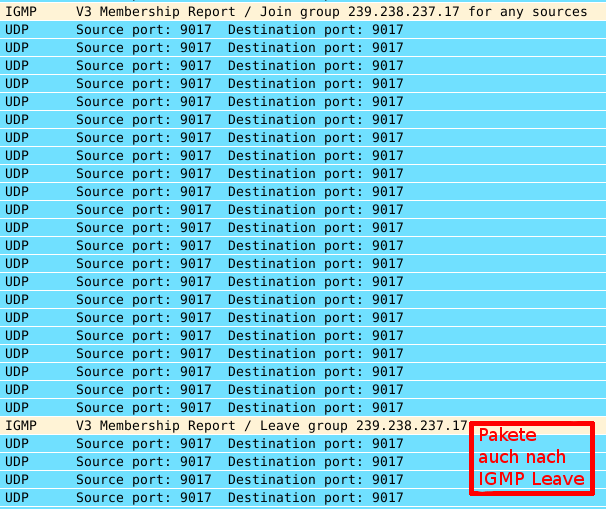
\includegraphics[width=0.6\textwidth]{multicast_after_leave.png}
	\end{center}

	\caption{IGMP Join/Leave bzgl. Ethernet-Ebene}

	\label{multicast_after_leave}
\end{figure}

Insofern hat das IGMP Join nur Auswirkungen auf den Stack des Hosts, 
der die IGMP-Join Nachricht abgesetzt hat.

\end{document}


